\identify{Identify the Challenge \& Set Goals: Arm V1.1 (September 28th, 2024)}
\info{Connor Albers}{Arm}{September 28th, 2024}
\chapterauthor{Connor Albers}
\label{chap:ArmV1.1}
\textbf{Goal}: We will identify an objective for our robot so that we can address it and build an effective solution
\section*{Problem Statement}
Our challenge was to create an effective arm mechanism for picking up rings while adhering to size constraints and ensuring functionality with existing components.

\section*{Solution Requirements}
\begin{itemize}
    \item The arm must be able to pick up rings reliably.
    \item It should fit within the robot's starting size.
    \item The mechanism must minimize motor usage due to limited availability.
\end{itemize}

\section*{Solution Goals}
\begin{itemize}
    \item Achieve a minimum of 80\% efficiency in ring pickup.
    \item Maintain a simple and effective design.
\end{itemize}


\brainstorm{Brainstorm \& Diagram: Arm V1.1 (September 28th, 2024)}
\info{Connor Albers}{Arm}{September 28th, 2024}
\chapterauthor{Connor Albers}
\section*{Possible Solution - Victory Arm}
One design in particular that caught our attention was 1168A, Victory’s arm. As shown in our bibliography: "\cite{1168APitsandParts}"
Their design used the same arm design as the redirect we had already constructed but swapped the basket and accompanying pneumatic with a simple claw.
\begin{figure}[H]
    \centering
    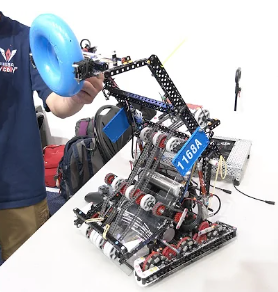
\includegraphics[width=0.5\linewidth]{images/Victory Arm Pits and Parts Thumbnail.png}
    \caption{\cite{1168APitsandParts}}
    \label{fig:1168A}
\end{figure}

\noindent
\textbf{Pros}:
\begin{itemize}
    \item Utilizes pneumatics, freeing up motors for other mechanisms.
    \item Greater leverage and range of motion.
\end{itemize}
\textbf{Cons}:
\begin{itemize}
    \item Potentially complex pneumatic setup.
    \item Requires careful positioning to avoid interference with the intake mechanism.
\end{itemize}

\section*{Possible Solution - Net Mechanism}
A "Net" Mechanism would take the Ring off of our Intake, using something similar to a catapult 

\begin{figure}[H]
    \centering
    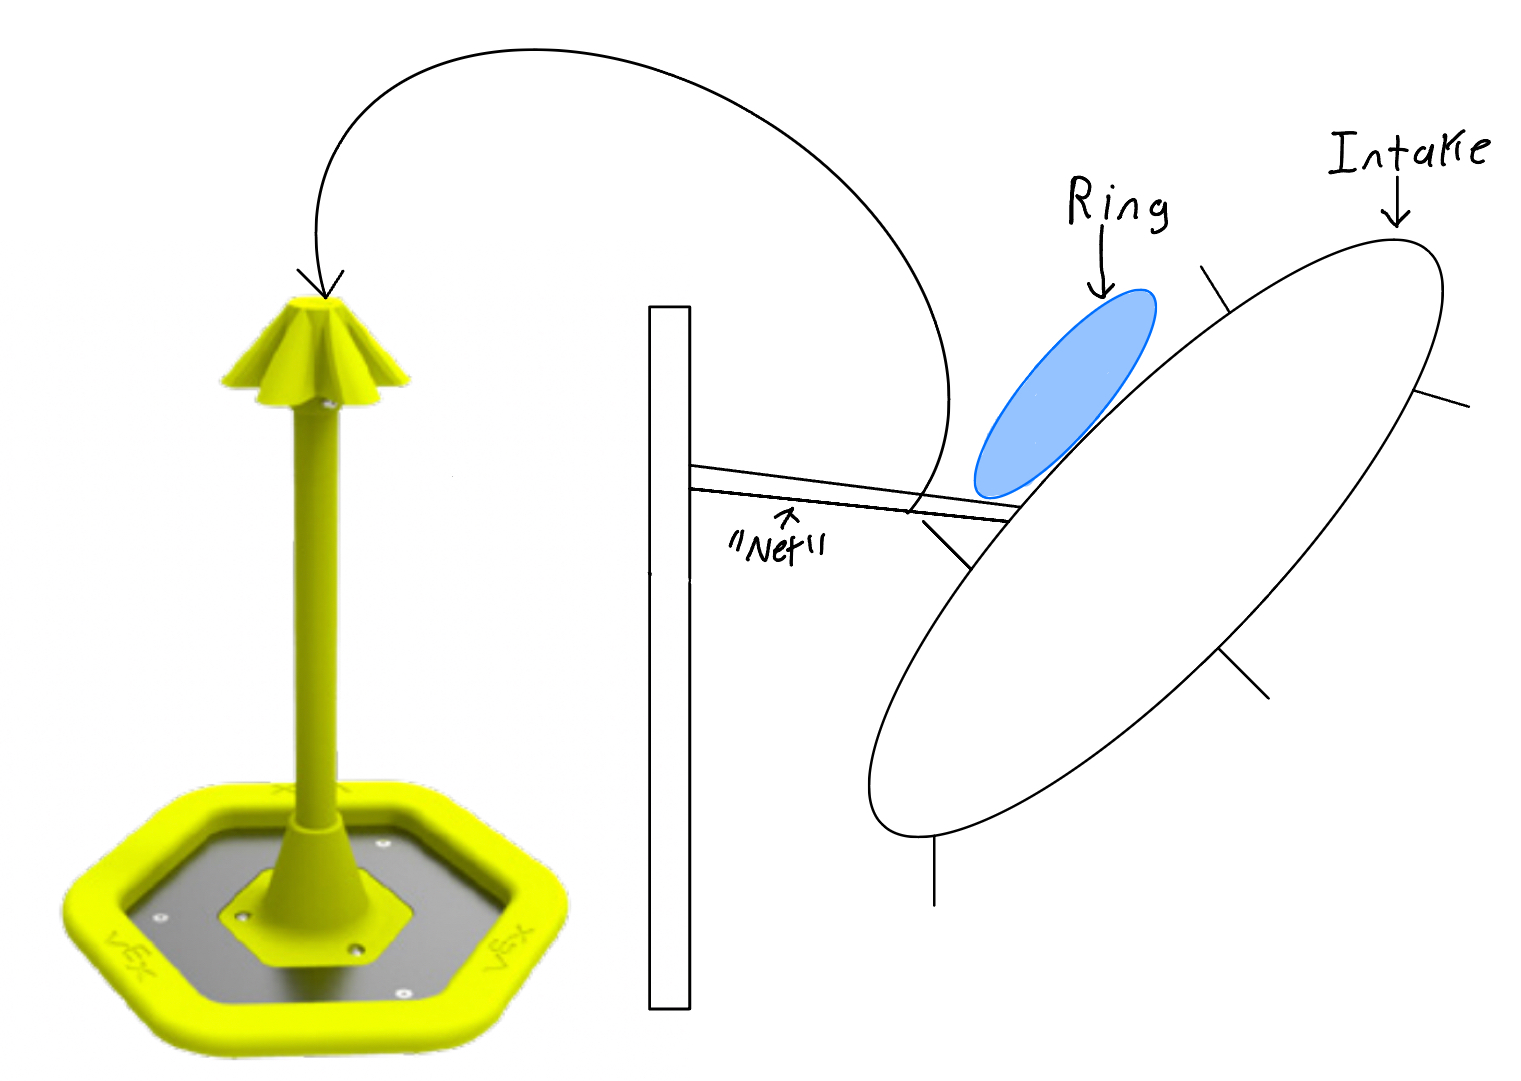
\includegraphics[width=0.5\linewidth]{images/Fishmech.jpg}
    \caption{Net Mechanism}
    \label{fig:fish-mech}
\end{figure}

\noindent
\textbf{Pros}:
\begin{itemize}
    \item Utilizes pneumatics.
    \item Greater leverage and range of motion.
    \item Very simple build
\end{itemize}
\textbf{Cons}:
\begin{itemize}
    \item Requires careful positioning to avoid interference with the intake mechanism.
\end{itemize}

\solution{Choose a Solution: Arm V1.1 (September 29, 2024)}
\info{Connor Albers}{Arm}{September 29th, 2024}
\chapterauthor{Connor Albers}
\section*{Choose a Solution}
\renewcommand{\arraystretch}{1.85} % Change this value as needed
\begin{table}[htb!]
\centering
\begin{tabular}{|>{\centering\arraybackslash}m{1.85cm}|>{\centering\arraybackslash}m{1.85cm}|>{\centering\arraybackslash}m{1.85cm}|>{\centering\arraybackslash}m{1.85cm}|>{\centering\arraybackslash}m{1.85cm}|>{\centering\arraybackslash}m{1.85cm}|>{\centering\arraybackslash}m{1.85cm}|}
\hline
\textbf{Scale 1 - 10} & \textbf{Simplicity} & \textbf{Reliability} & \textbf{Traction} & \textbf{Size} & \textbf{Speed} & \textbf{Total} \tabularnewline
\hline
Weight & x1 & x3 & x2 & x1 & x3 & \tabularnewline
\hline
Net Mechanism & 5 & 10 & 6 & 10 & 6 & 75 \tabularnewline
\hline
Victory Arm & 3 & 10 & 10 & 10 & 6 & 81 \tabularnewline
\hline
\end{tabular}
\caption{Arm Decision Matrix}
\label{tab:drive-matrix}
\end{table}
\renewcommand{\arraystretch}{1.85} % Reset to default
According to our point totals it seems that we will use 1168A, Victory's Arm. Lets make a plan in CAD. 
\section*{Make a Plan}
\begin{figure}[H]
    \centering
    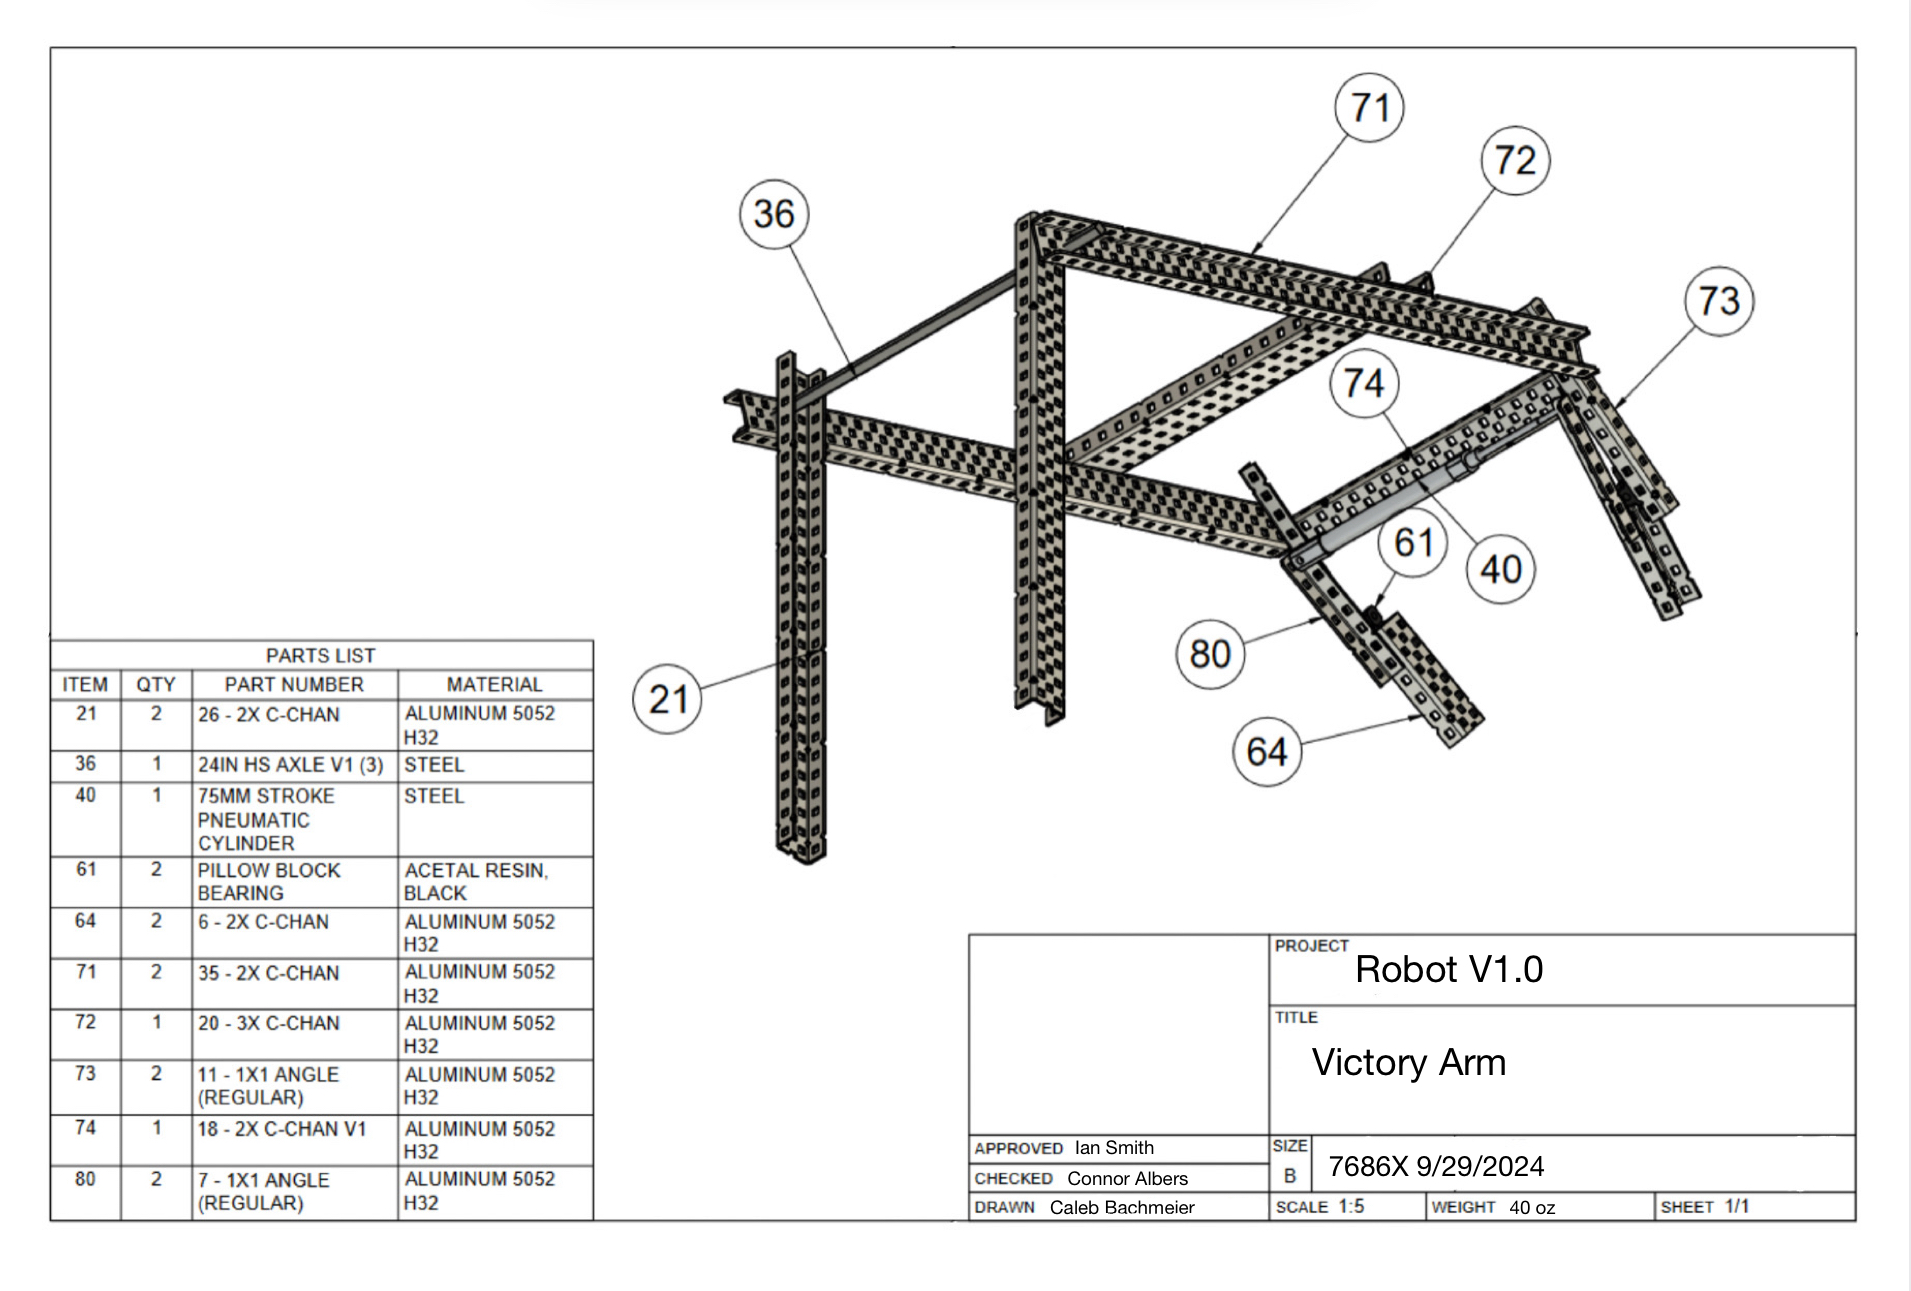
\includegraphics[width=1\linewidth]{images/Arm Drawing.jpg}
    \caption{Fusion 360 Arm Drawing}
    \label{fig:arm-drawing}
\end{figure}
\build{Build \& Program: Arm V1.1 (September 29th, 2024)}
\info{Connor Albers}{Arm}{September 29th, 2024}
\chapterauthor{Connor Albers}
\section*{Building}
\section*{Disassembly}
To start, we took off our basket and the pneumatic attached to it. 

\section*{Arm Modification}
Next, we swapped out the two main C-channels on the arm for full-length 35-hole ones.

\section*{Engineering the Claw}
The next step was to engineer the claw. Much like our previous design, the claw pivoted at the end of our arm but, unlike our previous design, it used rubber bands to force it out. 

The reason the claw needed to pivot was because it was at the front of our robot, meaning it would be hit every time we ran into something, which happens often during competition. Allowing the claw to pivot meant that every time we hit something, the claw would be pushed into the high-strength axle across our intake, and all the force would be transferred into it rather than into the arm itself.

\section*{Using L-Channels}
We used L-channels as the pieces that pivoted on the end of the arm (see Figure~\ref{fig:ichannelsendofarm}) because of their lightweight construction. Making our arm as light as possible was crucial to ensuring our arm would still work at lower air pressures. 

\begin{figure}[H]
    \centering
    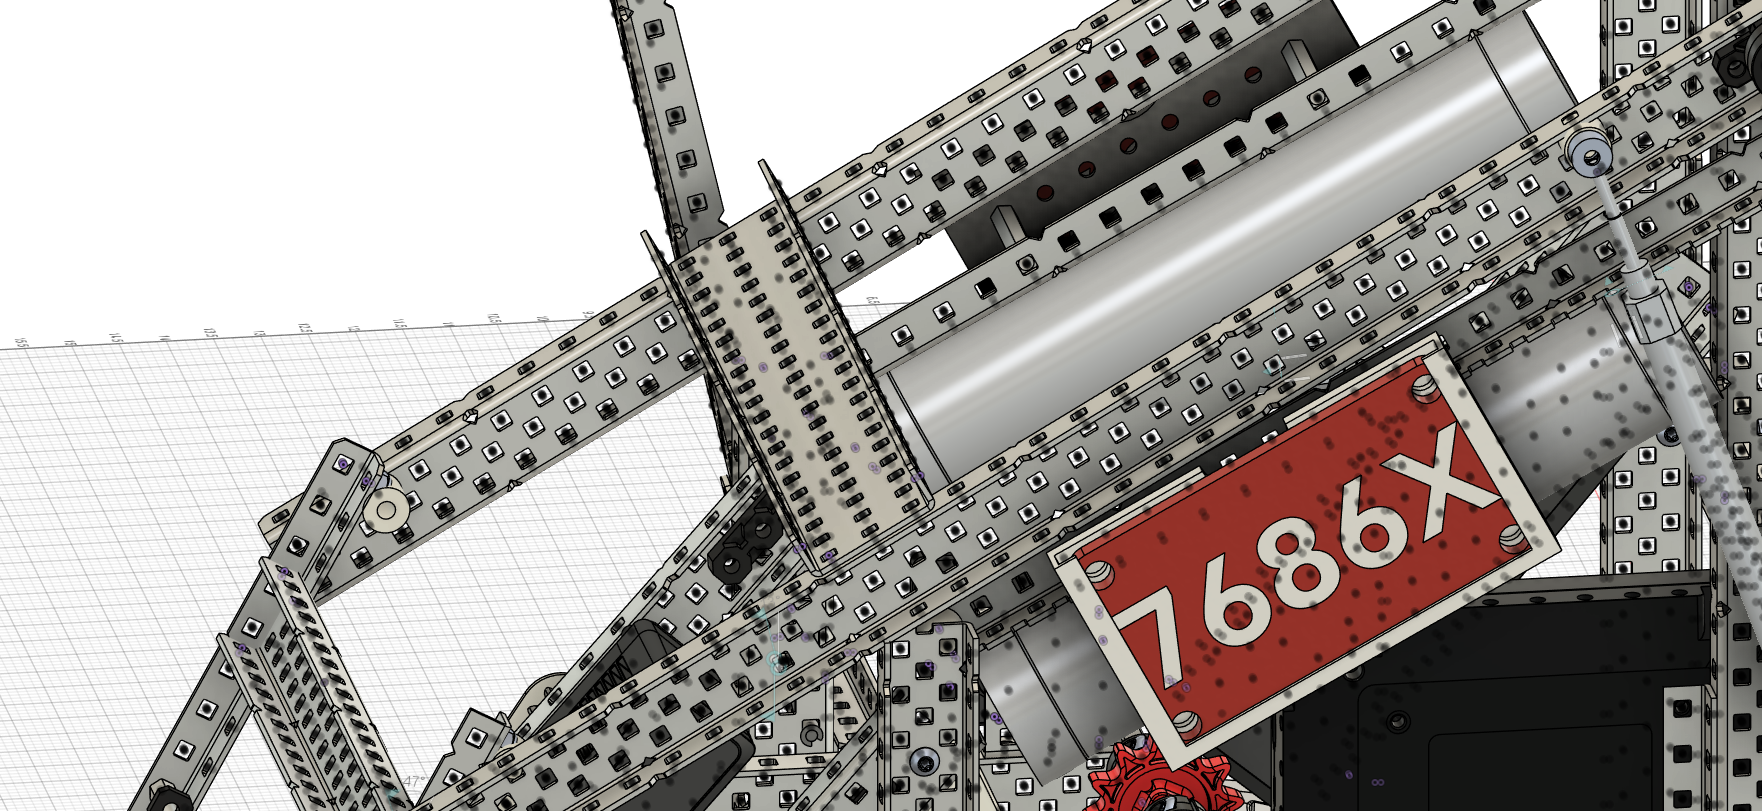
\includegraphics[width=0.7\textwidth]{images/Ichannelsendofarm.png}
    \caption{L-channels at the end of the arm.}
    \label{fig:ichannelsendofarm}
\end{figure}

By attaching pillow bearings to the L-channels (see Figure~\ref{fig:pillowbearings}), we were able to provide a spot for each side of our claw to pivot on. 

\begin{figure}[H]
    \centering
    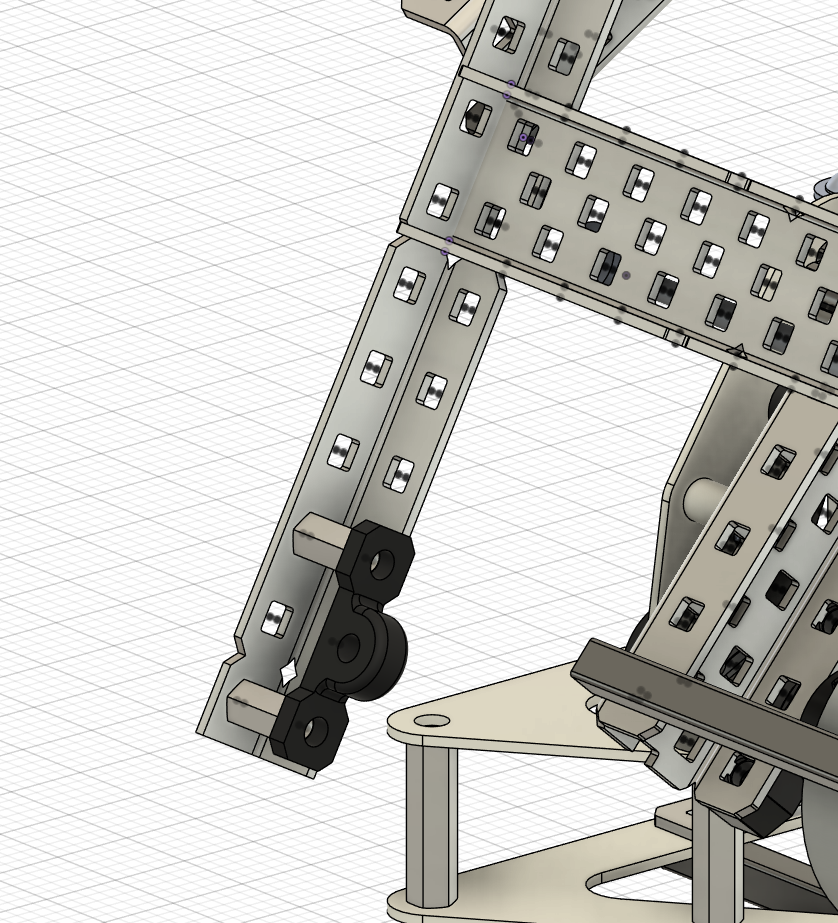
\includegraphics[width=0.7\textwidth]{images/Pillowbearings.png}
    \caption{Pillow bearings attached to L-channels.}
    \label{fig:pillowbearings}
\end{figure}

\section*{Claw Construction}
Each “finger” of the claw was constructed using a 1x2 C-channel and an L-channel to provide mounting for our pneumatic (see Figure~\ref{fig:clawfinger}). 

\begin{figure}[H]
    \centering
     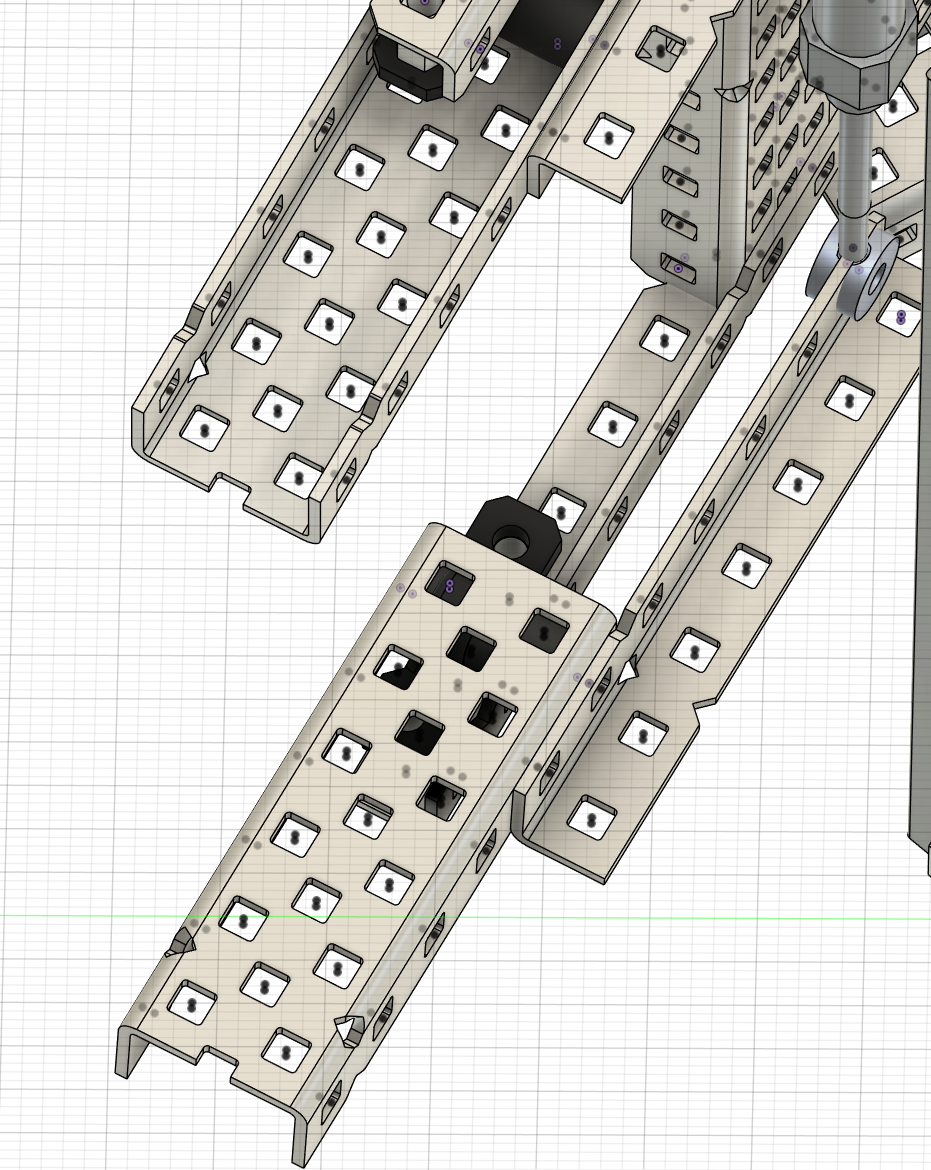
\includegraphics[width=0.7\textwidth]{images/clawfinger.png}
    \caption{Claw finger constructed with C-channel and L-channel.}
    \label{fig:clawfinger}
\end{figure}

\section*{Adding the Pneumatic}
The last step to complete our claw was to add the pneumatic. For this, we used a 50mm dual-action piston. After adding tubing and wiring to the pneumatic, our claw and arm assembly were completed.
%Add subsections about different building parts 
\test{Test the Solution: Arm V1.1 (September 30th, 2024)}
\section*{Test the Solution}